\section{Backend API}
In order to provide an interface for interacting with Neo4J, and to implement complex functionality such as clustering and path finding, I developed a backend API to support the features of the front end web application as described in section \ref{section-investigation-tool}. 

\subsection{Technology Choices}
The API was developed in Java using Spring Data as the predominant library used for communicating with Neo4J. 
\\\\
Spring Data provides powerful repository and object-mapping abstractions that can be used to define a data model and interact with the underlying data store through abstractions with relative ease. Spring Data has specific support for Neo4J, utilised by creating a repository that extends their \texttt{Neo4JRepository<>} interface. Spring Data repositories does much of the heavy lifting for you with query generation; queries will be derived from the repository method names that are defined. Spring Data also has support for many other underlying data repositories, such as MongoDB, Redit or Apache Cassandra. This would allow for the flexibility of changing the core underlying data store, or for new data sources from different types of data stores to be introduced.

\subsubsection{Alternative Technologies}
An alternative technology choice, which is often a popular approach, would be to create the API using Python Flask. This was considered and was an almost equal candidate for technology choice but I ultimately decided to choose Java \& Spring Data due to the huge community that exists for Spring MVC and its excellent documentation. Additionally, I was aware of the future potential of integrating Max Baylis Health Monitoring project [see \ref{background-max-baylist-project}] (written in Java) with my interface to Neo4J, in which case implementing the back-end in Java using Spring Data would make such an integration far easier. 


\subsection{API Design}
The API follows a REST design pattern; generally, ID's used to GET an entity are a path variable. Any further options such as data required for filtering exist as an optional query parameter.  

\begin{lstlisting}[label={lst:address-api}, caption={Get an address using the unique full address. Several optional query parameters for filtering by time, price and enabling clustering and node limiting. \\[0.5cm] }, breaklines=true, basicstyle=\small]
GET /bitcoin/address/{address | string}
    ?startTime={time filter start since epoch | string}
    &endTime={time filter end since epoch | string}
    &startPrice={price filter start | double, as string}
    &endPrice={price filter end | double, as string}
    &priceUnit={currency units of price filter | string of 'btc', 'gbp', 'usd' or 'eur'}
    &inputClustering={true/false | boolean}
    &nodeLimit={node limit number | integer}
\end{lstlisting}

\begin{lstlisting}[caption={Get an entity using the unique name of the entity . All query parameters are optional for filtering.}, breaklines=true, basicstyle=\small]
GET /bitcoin/entity/{entity name | string}
    ?startTime={time filter start since epoch | string}
    &endTime={time filter end since epoch | string}
    &startPrice={price filter start | double, as string}
    &endPrice={price filter end | double, as string}
    &priceUnit={currency units of price filter | string of 'btc', 'gbp', 'usd' or 'eur'}
    &nodeLimit={node limit number | integer}
\end{lstlisting}

\begin{lstlisting}[caption={Get an output with a unique output ID. All query parameters are optional for filtering.}, breaklines=true, basicstyle=\small]
GET /bitcoin/output/{output id | string}
    ?startTime={time filter start since epoch | string}
    &endTime={time filter end since epoch | string}
\end{lstlisting}

\begin{lstlisting}[caption={Get a transaction with a unique transaction ID (txid). All query parameters are optional for filtering.}, breaklines=true, basicstyle=\small]
GET /bitcoin/transaction/{transaction id | string}
    ?startTime={time filter start since epoch | string}
    &endTime={time filter end since epoch | string}
    &startPrice={price filter start | double, as string}
    &endPrice={price filter end | double, as string}
    &priceUnit={currency units of price filter | string of 'btc', 'gbp', 'usd' or 'eur'}
    &nodeLimit={node limit number | integer}
\end{lstlisting}

\begin{lstlisting}[caption={Get a block with a unique block hash}, breaklines=true, basicstyle=\small]
GET /bitcoin/block/{block hash}
\end{lstlisting}

\begin{lstlisting}[caption={Find a path between two addresses using their full address strings}, breaklines=true, basicstyle=\small]
GET /bitcoin/shortestPath/{start address}/{end address}
\end{lstlisting}

\subsubsection{Responses}
A typical response will contain all information for the requested entity, and its immediate neighbours. For example, the request \\\texttt{GET /bitcoin/address/1261hwCRfSEA8qLkVhLYS2a3CFzegiUxGU} will have the response shown in listing \ref{lst:output-response}. The start and end nodes are fully defined, and each intermediate node on the path (each potentially of a different type) are included in the \texttt{intermediateNodes} array, with the links that connect each of the nodes included in the \texttt{rels} array. 

\begin{lstlisting}[label={lst:output-response}, caption={GET Output Example Response}, breaklines=true, basicstyle=\small]
{
    "outputId": "fbec1c21ca91d4e5baf55f305b05d294755b4fd069d149344b2104b708e42873-0",
    "value": 50,
    "producedByTransaction": {
        "transaction": {...}
        "eurValue": 0,
        "usdValue": 0,
        "gbpValue": 0,
        "timestamp": 1232709019
    },
    "inputsTransaction": {
        "transaction": {...},
        "eurValue": 0,
        "usdValue": 0,
        "gbpValue": 0,
        "timestamp": 1233004161
    },
    "lockedToAddress": {
        "address": {
            "address": "1BENJudbbZ8dfTwFtCLuJNWMTtBLE2bZa",
            "entity": null,
            "hasLinkedAddresses": true
        }
    }
}
\end{lstlisting}

The response for the path finder method takes on a different format. For example, executing the path finding query on addresses \textit{1CrnUia9wfeNFbdwKJNj89YqA6qetvYTTE} and \texttt{17c6L9JUGVenn6CfqXuB93L3Tk8Tbzefui} returns the response showwn in listing \ref{lst:path-find-response}.

\begin{lstlisting}[label={lst:path-find-response}, caption={Response to a path find query}, breaklines=true, basicstyle=\small]
[
    {
        "startNode": {
            "address": "1CrnUia9wfeNFbdwKJNj89YqA6qetvYTTE",
            "outputs": [
                {...}
            ],
            "entity": null,
            "inputHeuristicLinkedAddresses": null,
            "hasLinkedAddresses": false
        },
        "intermediateNodes": [
            {...},
            {...},
            {...}
        ],
        "rels": [
            {...},
            {...},
            {...}
        ],
        "endNode": {
            "address": "17c6L9JUGVenn6CfqXuB93L3Tk8Tbzefui",
            "outputs": [
                {...}
            ],
            "entity": null,
            "inputHeuristicLinkedAddresses": null,
            "hasLinkedAddresses": false
        }
    }
]
\end{lstlisting}

\subsection{Implementation} 
\subsubsection{Overall Design}
The API is created by the BitcoinController class. This is achieved using the Spring Data \texttt{@RestController} mapping under which the API exists under is created using the \texttt{@RequestMapping} annotation. Requests are handled by each of the methods shown on the BitcoinController class ion figure \ref{fig:backend-uml}. A request will be sent to the service which coordinates the data to be returned using a number of the repositories. There exists one repository for each type of entities. 

\begin{figure}
  \centering
  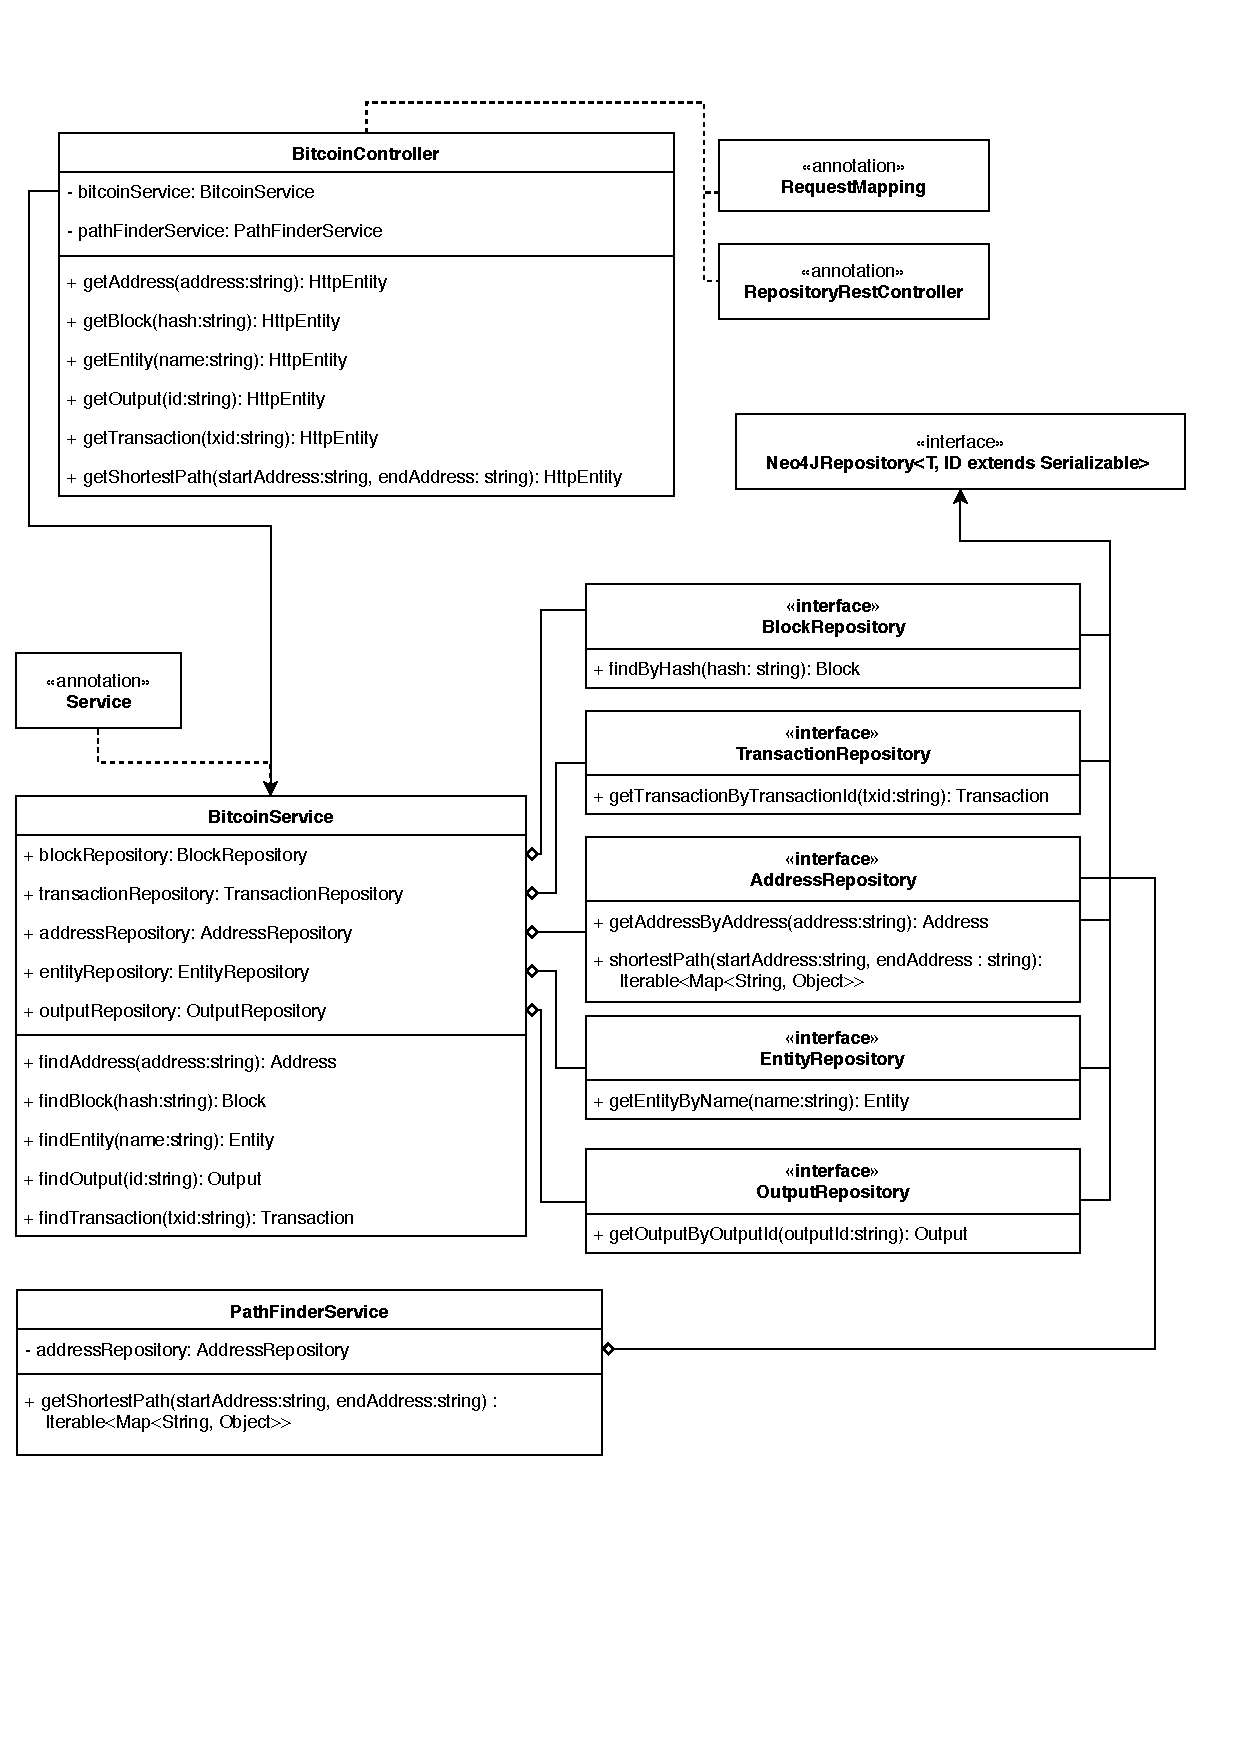
\includegraphics[width = 15cm]{./figures/backend-uml}\\[0.5cm] 
  \caption{Backend UML}
  \label{fig:backend-uml}
\end{figure}

\subsubsection{Node Entities}
Entities are defined as part of the data model using the Spring Data \texttt{@NodeEntity} annotation; Relationships from the database can be represented using the \texttt{Relationship} annotation. An example of a node entity class is the Transaction class; the implementation of the Transaction class can be seen in listing \ref{lst:node-entity-transaction}.
\\\\
\texttt{@NodeEntity} is used to tell Spring Data this class represents the data model of a node in Neo4J. The \texttt{@Id} annotation identifies the \texttt{id} field as the nodes unique identifier from Neo4J. \texttt{@Relationship} annotations are used to populate the model with the other nodes in the graph the Transaction node is connected to. 

\subsubsection{Serialising Node Entities}
The annotation \texttt{@JsonIgnoreProperties} is used to prevent infinite recursion when serialising responses to be returned by the API. For instance, if a Transaction references the Output node that it produces, and each Output references the Transaction node that produces it, the serialisation will indefinitely recurse until a stack overflow issue is encountered. Additionally, methods omitted from the listing for brevity are the Getter and Setter methods that exist for the properties; these methods help define the fields that should be serialised. For instance, no Getter exists for the \texttt{id} field since it is not required in the response. 

\begin{lstlisting}[language=Java, label={lst:node-entity-transaction}, caption={A transaction node entity}, breaklines=true, basicstyle=\small]
@NodeEntity(label = "TRANSACTION")
public class Transaction {
    @Id
    @GeneratedValue
    private Long id;

    private String transactionId;

    @Relationship(type = "MINED_IN", direction = Relationship.OUTGOING)
    private Block minedInBlock;

    @JsonIgnoreProperties("transaction")
    @Relationship(type = "INPUTS", direction = Relationship.INCOMING)
    private List<InputRelation> inputs;

    @JsonIgnoreProperties("inputsTransaction")
    @Relationship(type = "INPUTS", direction = Relationship.INCOMING)
    private Coinbase coinbaseInput;

    @JsonIgnoreProperties("transaction")
    @Relationship(type = "OUTPUTS")
    private List<OutputRelation> outputs;

}
\end{lstlisting}

\subsubsection{Implementing Repositories}
As shown in the UML diagram \ref{fig:backend-uml}, repositories all exist as interfaces which extend the \texttt{Neo4JRepository} interface. In doing so, many of the queries are automatically inferred based on the names of the methods defined on the interface. For example, the implementation of the AddressRepository interface is shown in listing \ref{lst:address-repository}. The method \texttt{getAddressByAddress} requires no query definition since Spring Data infers the query by the name of the method, and knows the type as the interface provides the \texttt{Address} type as one of the generic type arguments when extending Neo4jRepository. 
\\\\
Comparatively, the method shortestPath does require a query definition using the Spring Data \texttt{@Query} annotation; this is as the query is more specialised and cannot be inferred.

\begin{lstlisting}[language=Java, label={lst:address-repository}, caption={AddressRepository interface definition}, breaklines=true, basicstyle=\small]


public interface AddressRepository extends Neo4jRepository<Address, Long> {

    Address getAddressByAddress(@Param("address") String address);

    @Query("MATCH " +
            "(a1:ADDRESS{address:{0}}), " +
            "(a2:ADDRESS{address:{1}}), " +
            "p = shortestPath((a1)-[:INPUTS |:OUTPUTS |:LOCKED_TO*..100]-(a2)) " +
            "RETURN a1 as startNode, nodes(p) as intermediateNodes, relationships(p) as rels" +
            ", a2 as endNode")
    Iterable<Map<String, Object>> shortestPath(String sourceAddress, String destinationAddress);
}
\end{lstlisting}

\subsubsection{Implementing Path Finding}
The implementation of the path finding functionality can be seen in listing \ref{lst:address-repository}. Neo4J provides the method \texttt{shortestPath} that can be used to find a path between two nodes; I restricted the type of paths to be of type \texttt{INPUTS}, \texttt{OUTPUTS} or \texttt{LOCKED\_TO} in order for the path to represent the flow of funds, rather than paths existing simply due to the fact all addresses are connected via outputs that are spent in transactions that are mined in blocks which are chained from each-other.

